\documentclass[twocolumn]{aastex63}


\newcommand{\vdag}{(v)^\dagger}
\newcommand\aastex{AAS\TeX}
\newcommand\latex{La\TeX}

% \received{June 1, 2019}
% \revised{January 10, 2019}
\accepted{\today}
%% Command to document which AAS Journal the manuscript was submitted to.
%% Adds "Submitted to " the argument.
\submitjournal{AJ}

\shorttitle{Project Proposal}
\shortauthors{Hauch}

\begin{document}

\title{The Fate of Sun-like Stars Within M31 During Galactic Merger}
\author{Colin Hauch}


\section{Introduction} \label{sec:intro}
What is the fate of stars at the Sun's location (8 kpc from the center of the galaxy) but in M31's Disk? I am proposing to create a visualization of the night sky from the perspective of an observer on an M31 disk particle throughout the merger of M31 and The Milky Way Galaxy (MW). As part of this project, I would visualize the locations of various components of the original galaxies within the merged remnant.

Understanding how the merger between M31 and MW will transpire is important for us to understanding of galaxy mergers in general. Humanity's proximity to this particular merger allows precise observations to be made thus helping us better understand galactic dynamics. This project will attempt to provide a visualization of what the merger would appear to a sun-like system. We can use the results to make better models and predictions and better comprehend measurements of galactic dynamics. 

We currently understand that the two largest galaxies in the local group will likely collide in the future \citep[e.g.][and many others]{vdm12,vdm19}. Some publications document visualizations \citep{cox08}. However, I have not found a visualizations from the perspective of a planet in an M31 solar system that is in a sun-like position within M31 (8 kpc from the center of the galaxy). This is what I am hoping to create.

Where is our Sun likely to end up relative to what is left over after the M31-MW merger? This is one of the questions in the field that does not have a definite answer \citep{cox08}. There seems to be a huge variance in the "final" location of a sun-like system (see figure \ref{fig:sun}). I hope to learn more about how to determine and/or predict the fate of specific particles. 

\begin{figure}[htp]
    \centering
    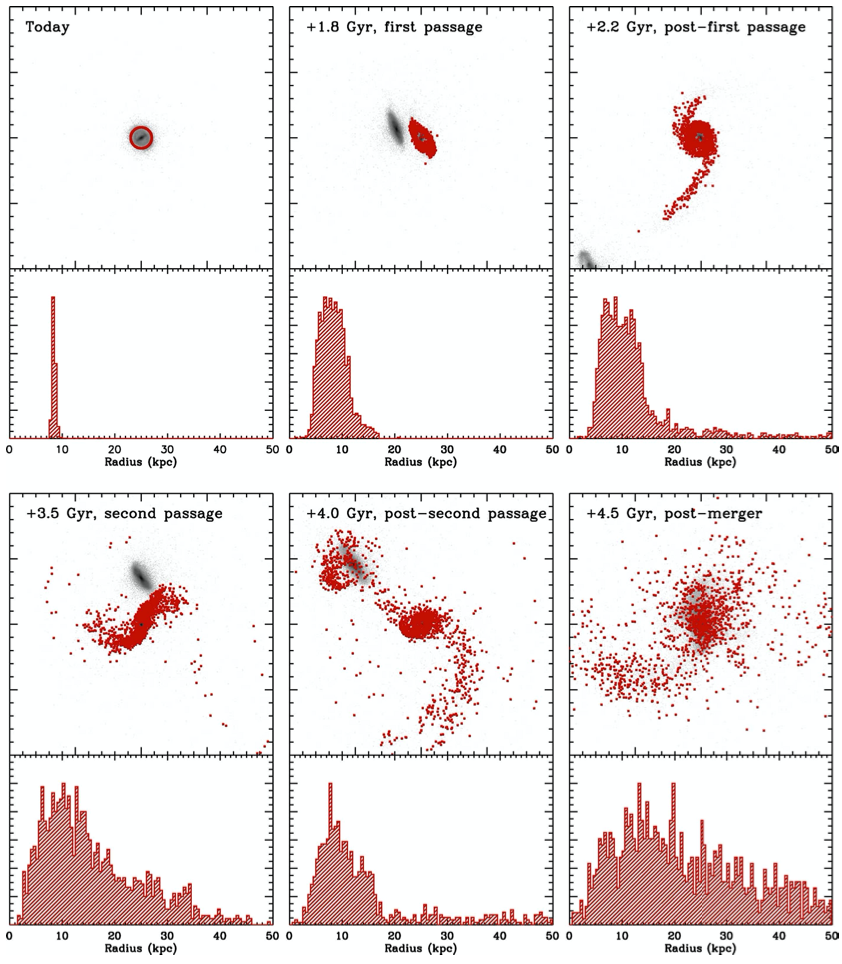
\includegraphics[width=2in]{sun.png}
    \caption{Figure directly from \cite{cox08}}
    \label{fig:sun}
\end{figure}

\section{The Proposal: Specific Questions} \label{sec:style}

\subsection{How will particles be selected?}
\emph{How will you select particles in M31/M33’s disk that are similar to the sun?} I will select particles within the disk of M31 that are some amount similar to the initial conditions of a sun-like system. A "similarity factor" (likely represented by a percentage) would be created for each relevant quantity: distance from center of galaxy and velocity vector. This similarity factor could be adjusted to allow for a larger or smaller tolerance on the similarity of a given particle to that of a determined sun-like system.  

\subsection{Which viewing orientations will be utilized?}
\emph{What kind of viewing orientations could you examine through visualizations? Image of night sky from perspective of particle, or from an outside observer? From another galaxy?} There are a number of viewing orientations of the merger that I believe would be enlightening. Specifically, the view of the night sky of a M31 sun-like system towards the center of mass of the MW. This would given an impression of what it would look like to experience the merger over the course of the entire simulation but would leave out an intuition for the merger. Another angle, from a fixed point relative to the motion of the galaxies, could provide that intuition.

\subsection{Why develop visualizations of simulation data?}
\emph{Why is it important to develop visualizations of simulation data sets?} Visualizations of simulations give us a foundation to hypothesise about and interpret observational data. Data sets are generally lists of parameters which are not particularly conducive to human understanding. Visualizations provide a medium through which to help understand the results of simulations in a more intuitive way.

\subsection{What properties could be examined?}
\emph{What kind of properties could you examine through visualizations?} A number of quantities would be interesting to actively track. For example, we could document a number of sun-like systems and their distance from the center of their home galaxies, as was done in \cite{vdm19}. Do they tend to migrate inwards or outwards? Is the magnitude of their velocity vector more likely to increase or decrease over the course of the merger? How often are sun-like systems ejected from the merger system? Each of these properties could be documented and could provide interesting results about the fate of our own solar system. \cite{vdm12} tracked a number of sun-like system candidates and created a histogram of their final displacements from the center of the M31-MW remnant (figure \ref{fig:hist}).

\begin{figure}[htp]
    \centering
    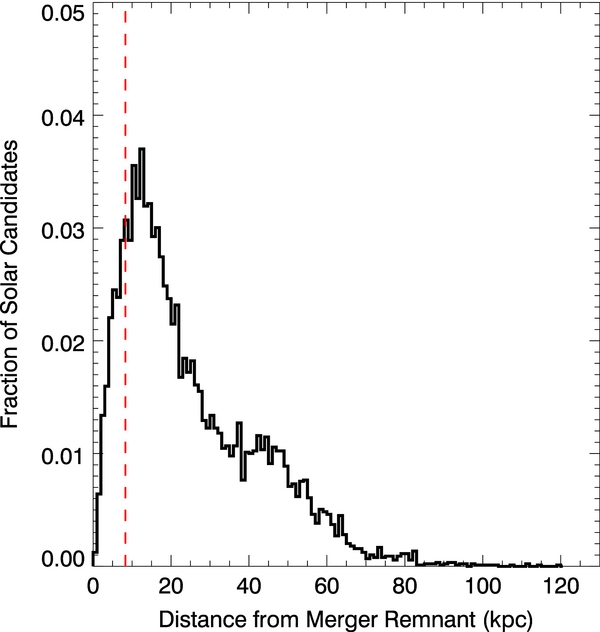
\includegraphics[width=2in]{hist.jpg}
    \caption{Figure directly from \cite{vdm12}}
    \label{fig:hist}
\end{figure}

\subsection{Which visualization formats will be used?}
\emph{Are you thinking to make movies? Or still shots?} I am proposing making a series of movies, with still shots taken from individual frames of these movies to add clarity when movies are not an option. I think movies will give a better intuition for the visualization than still shots would give; I do however recognize that a movie format is not always an option when presenting results. I hope to provide a combination of both still shots and short movies.

\subsection{Tools available?}
\emph{What kind of tools do you already know how to use, or what are you planning to learn how to use?} I have previous experience with the matplotlib, a python plotting library. I believe this tool could be used to create the visualizations. 

\subsection{Technical approach to the problem}
\emph{How will you approach the problem using the simulation data? Outline the codes you'd need to write in general terms.} First, select a number of sun-like system candidates from the M31 disk. Perhaps they can be ranked in order of similarity to relevant sun parameters. This would also be the time to somehow mark particles; maybe they can be color-coded to indicate initial location or velocity. Next, fully simulate the data set for some period of simulated-time. Finally, plot a series of stills from this simulation at specified intervals and extract them. These stills can then be used as single images and can be combined to create a movie.

\subsection{Hypothesis of what will be found}
\emph{What is your hypothesis of what you will find? Why do you think this will occur?} I expect to create a visualization the provides some sense of spacial intuition for the collision between M31 and the MW. I expect the result to be visually interesting but otherwise not particularly scientifically significant. I expect predictions of individual systems will be nearly impossible as it seems that both galaxies mix with each other significantly: they merge. However, gaining some kind of intuition for the nature of the merger could shine light on the system as a whole and inspire some to take a more data/result driven approach to this incredible merger event.



\bibliography{demo}{}
\bibliographystyle{aasjournal}

\end{document}
